\documentclass[a4paper,12pt,singlespacing]{article}
% Arquivo de configurações do modelo
\usepackage[T1]{fontenc}
\usepackage[utf8]{inputenc}
\usepackage[lmargin=2cm, rmargin=2cm, tmargin=2.5cm, bmargin=2.5cm]{geometry}
\usepackage[brazil, brazilian]{babel}
\usepackage[style=abnt]{biblatex}
\usepackage[pdftex]{hyperref}
\usepackage{csquotes, graphicx, xcolor, comment, enumerate, multirow, multicol, titlesec, amsmath, amsthm, amsfonts, amssymb, dsfont, mathtools, blindtext, ragged2e, array, enumitem, tikz, bbding, pifont, wasysym, amssymb, hyperref, titling}
\newcommand{\cmark}{\ding{51}}
\newcommand{\xmark}{\ding{55}}
\usepackage{float}

\tolerance=1
\emergencystretch=\maxdimen
\hyphenpenalty=10000
\hbadness=10000

\usepackage{helvet}
\renewcommand{\familydefault}{\sfdefault}

\usepackage{setspace}
\setlength{\JustifyingParindent}{1.25cm}
\setlength{\RaggedRightParindent}{0pt}
\setlength{\parskip}{6pt}

\usepackage{fancyhdr}
\pagestyle{fancy}
\fancyhf{}
\lhead{}
\rhead{}
\rfoot{\small\thepage}
\renewcommand{\headrulewidth}{0pt}

\titlespacing*{\section}{0pt}{6pt}{0pt}
\titlespacing*{\subsection}{0pt}{6pt}{0pt}
\titlespacing*{\subsubsection}{0pt}{6pt}{0pt}

\renewcommand{\thesection}{\arabic{section}.}
\renewcommand{\thesubsection}{\arabic{section}.\arabic{subsection}.}
\renewcommand{\thesubsubsection}{\arabic{section}.\arabic{subsection}.\arabic{subsubsection}.}

\titleformat{\section}{\normalsize\bfseries}{\makebox[1.25cm][l]{\thesection}}{0pt}{}
\titleformat{\subsection}{\normalsize\bfseries}{\makebox[1.25cm][l]{\thesubsection}}{0pt}{}
\titleformat{\subsubsection}{\normalsize\bfseries}{\makebox[1.25cm][l]{\thesubsubsection}}{0pt}{}

\usepackage{textcase}
\usepackage[font=small, labelsep=endash, textfont=bf, labelfont=bf, aboveskip=6pt, belowskip=-6pt, tablename=TABELA, figurename=FIGURA]{caption}
\usepackage[font=small, labelsep=endash, textfont=bf, labelfont=bf, aboveskip=6pt, belowskip=3pt, labelformat=simple]{subcaption}

\renewcommand{\thetable}{\arabic{table}}
\renewcommand{\thefigure}{\arabic{figure}}
\renewcommand{\thesubfigure}{\arabic{subfigure}}
\renewcommand{\thesubtable}{\arabic{subtable}}

\addbibresource{ref.bib}

% Utilizado para correções e comentários. Vá para 'util.tex' para saber mais.
\include{util}

% Aqui devem ser inseridas as informações sobre o trabalho
    % Título:
    \title{Relatório do projeto de admissão}
    % Alunos e orientadores:
    \author{Ana Carolina (acsd@ufpi.edu.br)}

\begin{document}
    {\centering
        \setlength{\parskip}{0pt}
        Pontifícia Universidade Católica do Rio Grande do Sul - PUCRS
        
        \setlength{\parskip}{0pt}
        DELL - IT Academy

        \setlength{\parskip}{18pt}
        \textbf{ \thetitle }
        \setlength{\parskip}{12pt}
        
        \theauthor
        
        \setlength{\parskip}{6pt}
        
    }

    \justifying
    
%    \tableofcontents
%    \newpage
    
    \section{Resumo geral do projeto}
Em 10 de junho de 2021, foi enviado um exercício prático com fins avaliativos para a admissão no programa DELL IT Academy. O exercício consiste na criação de um programa, em qualquer linguagem, para implementar as seguintes funcionalidades:
\begin{itemize}
    \item Listar todos os pontos de táxi da tabela CSV anexa;
    \item Informar um par de coordenadas para que possa ser efetuada uma;
    \item Busca de pontos próximos a essas coordenadas;
    \item Busca de pontos de táxi por logradouro; e
    \item Encerramento do programa.
\end{itemize}


\section{Sobre a linguagem utilizada}
Escolhi a linguagem Python para poder aprender mais sobre ela enquanto crio meu programa. No início do período, estava engajada em aprender os comandos básicos (print, input, entre outros) e tentar desenvolver alguns projetos básicos mas, com o tempo passando e as provas da universidade e outros projetos tomando conta da minha agenda, resolvi deixar de lado.

Python é uma linguagem open-source de propósito geral. Desde o Ensino Médio, é um dos meus pontos de interesse em computação, sendo inclusive um dos motivos que tive para ingressar no curso de Ciência da Computação em 2019 e comparecer à conferência Python Nordeste com alguns amigos, no mesmo ano.

Por causa de sua flexibilidade e possibilidade de integração com outras linguagens e frameworks, ela chama a atenção e não deixa de ser assunto em rodas de desenvolvedores. Uma das pessoas nas quais me inspiro no meu curso a utiliza bastante, e ela sempre disse que seu lema é 'aprender ensinando'. Isso foi o suficiente para me convencer a utilizar essa linguagem no meu exercício.


\section{Sobre o programa desenvolvido}
Tentei resumir minha submissão a um arquivo em Python (.py) e a tabela CSV enviada como anexo junto ao exercício, além deste relatório. Começo definindo minha autoria e a data de finalização do código. Em seguida, as importações de módulos: csv para leitura do arquivo anexo, sys para alguns comandos relacionados ao ambiente em que o Python está rodando, e partes de math para os comandos matemáticos exigidos pela função haversine. 

Grande parte do programa está dentro da classe Main, que é executada no fim do arquivo PY. A primeira parte consiste em uma função \_\_init\_\_, que lê o arquivo CSV através da próxima função, lerArquivo; remove o cabeçalho para uma melhor visualização dos dados; e lista todas as opções do menu, como pedido na especificação da atividade. Após realizar essas ações, a localização que o usuário irá digitar posteriormente é definida como lista, ou vetor.

A função lerArquivo, como supracitado, define os pontos de táxi como uma lista, abrindo e lendo o arquivo CSV, separando seus valores com 'enter' e ponto-e-vírgula, para que possa retorná-los e que as outras funções o possam utilizar de forma menos problemática. O menu principal é impresso de acordo com as especificações em \_\_init\_\_, e a entrada do usuário para escolher a função a ser executada é verificada até que ele digite uma opção válida. Ao fim da função, é determinada a próxima a ser executada.

A primeira função propriamente especificada a ser implementada foi a de listar todos os pontos de táxi cadastrados. Para isso, a organização prévia da tabela foi aproveitada e adequadamente impressa, com um cabeçalho mais organizado e com iniciais maiúsculas, contrastando com as do arquivo CSV original. Após a execução, retorna-se ao menu principal.

A próxima função é aquela onde o usuário informa sua localização (ou qualquer par ordenado de coordenadas dentro do que é possível ter: latitude entre -90 e +90, longitude entre -180 e +180). São feitas validações da localização dada, e se o usuário digitar o valor com vírgula, como no CSV, esta é prontamente trocada por um ponto, para facilitar operações como float. Caso isso não seja possível, é dado um aviso de 'formato inválido', assim como nas próprias coordenadas digitadas. Ao fim da execução dessa função, mais uma vez retorna-se ao menu principal.

A terceira função é a de encontrar pontos próximos à localização digitada. Para isso, verificou-se se o vetor (definido em \_\_init\_\_) foi preenchido, ou seja, se existem coordenadas cadastradas no sistema. Caso não hajam, o usuário retorna ao menu principal. Caso hajam, segue a execução, calculando a distância de cada ponto cadastrado à localização digitada, através da fórmula de haversine, dada nas especificações da tarefa. Mais uma vez, há a substituição de vírgulas por pontos para um melhor funcionamento. A seguir, os três pontos mais próximos são listados, à direita de suas respectivas distâncias à localização do usuário, em forma de tabela. Retorna-se ao menu mais uma vez.

Na função seguinte, procuramos pontos de táxi por digitação de substring parecida com o logradouro desejado. Há uma validação found, que equivale à pergunta 'Algum logradouro já foi encontrado?', e há a utilização constante de print() para pular linhas e deixar o código mais organizado. É pedido que o usuário digite 'todo ou parte do nome do logradouro' a ser pesquisado, pois a string resultante da pesquisa será colocada em letras maiúsculas (uppercase) e comparada com logradouros de toda a tabela de pontos para que se tente encontrar um logradouro cujo nome 'bata' com esta string de alguma forma, seja parcial ou totalmente. Caso esses logradouros sejam encontrados, é criada e impressa, em forma de tabela, uma lista com eles. Caso contrário, é informado ao usuário. Retorna-se ao menu principal mais uma vez.

A última função, 'quit\_system' ou 'fechar sistema', em português, dá um pequeno aviso e faz sua tarefa homônima. Nas últimas linhas do arquivo, especifico a função haversine, que funciona com cálculos envolvendo dois pares de coordenadas e o raio do planeta Terra, retornando este raio vezes a fórmula calculada nas variáveis 'a' e 'c'. Na última linha, a função menu é chamada pela primeira vez, para que, ao executar o arquivo PY, o programa funcione apropriadamente.

\newpage
\section*{Anexo 01: Capturas de tela da execução de cada função}

\begin{figure}[!h]
    \centering
    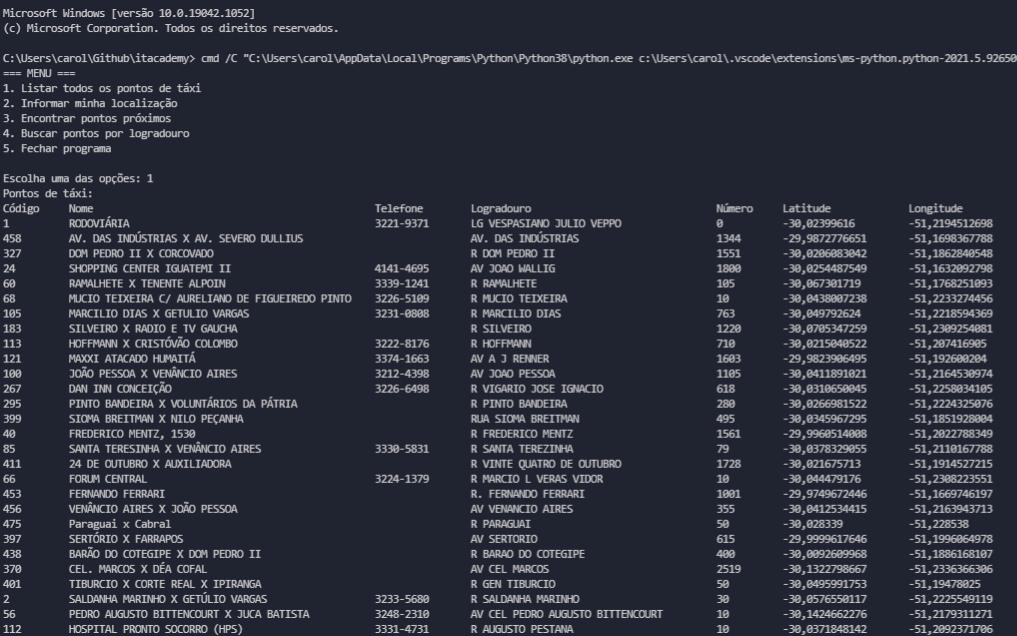
\includegraphics[width=0.7\textwidth]{artigo/img/1.PNG}
    \caption{Função 'Listar pontos de táxi'}
    \label{fig:my_label}
\end{figure}

\begin{figure}[!h]
    \centering
    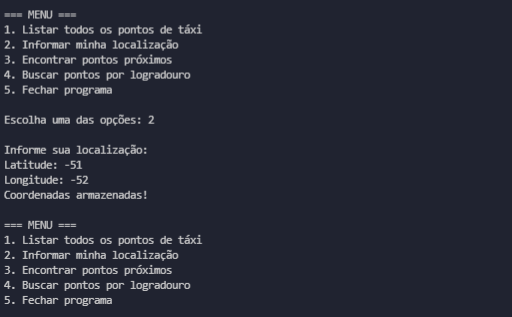
\includegraphics[width=0.7\textwidth]{artigo/img/2.PNG}
    \caption{Função 'Informar localização'}
    \label{fig:my_label}
\end{figure}

\begin{figure}[!h]
    \centering
    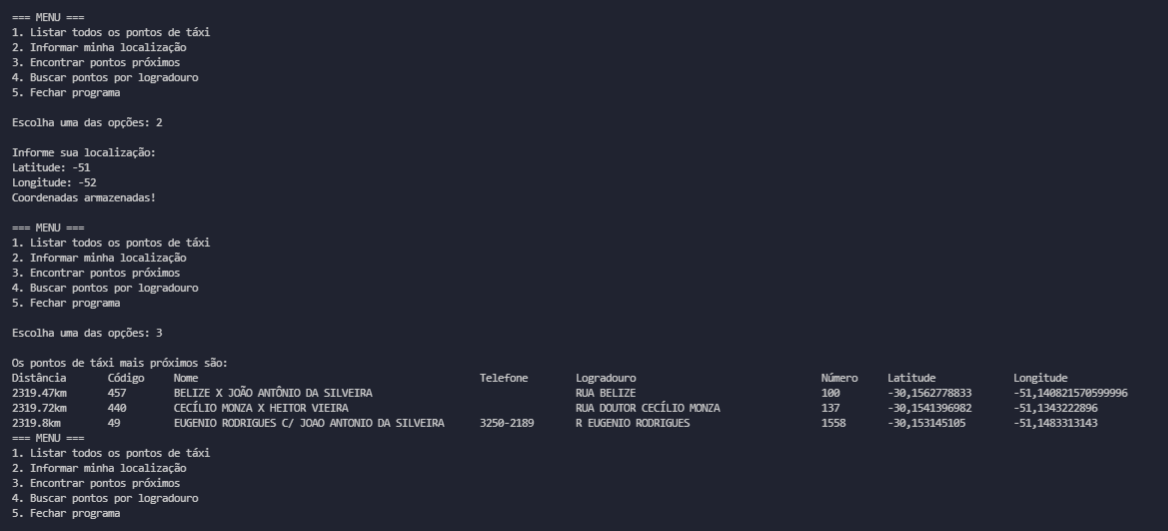
\includegraphics[width=0.7\textwidth]{artigo/img/3.PNG}
    \caption{Função 'Encontrar pontos próximos'}
    \label{fig:my_label}
\end{figure}

\begin{figure}[!h]
    \centering
    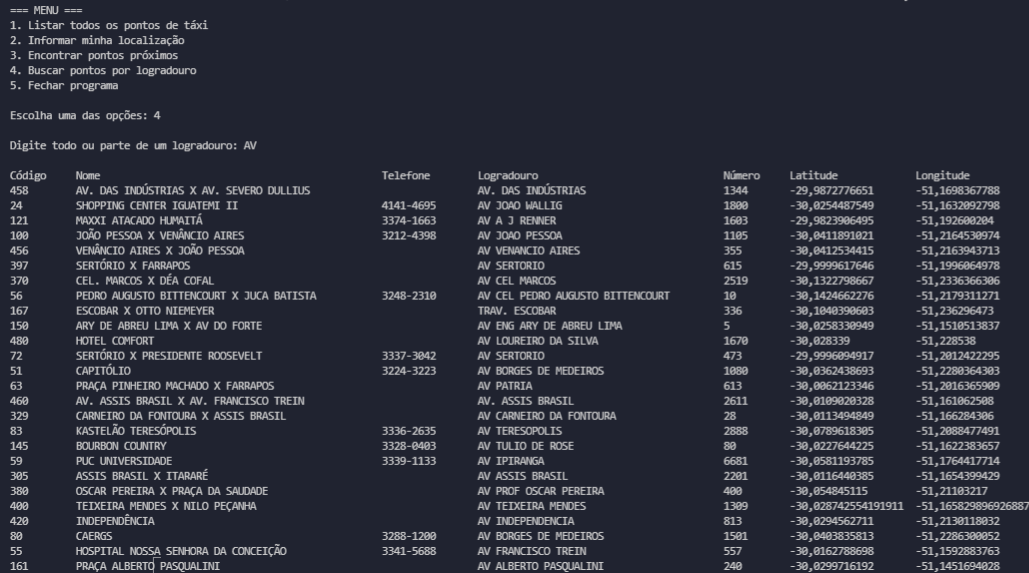
\includegraphics[width=0.7\textwidth]{artigo/img/4.PNG}
    \caption{Função 'Buscar por logradouro'}
    \label{fig:my_label}
\end{figure}

\begin{figure}[!h]
    \centering
    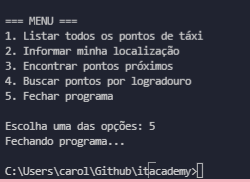
\includegraphics[width=0.7\textwidth]{artigo/img/5.PNG}
    \caption{Função 'Encerrar'}
    \label{fig:my_label}
\end{figure}

\section*{Considerações finais}
\begin{itemize}
    \item Esse é o meu primeiro programa em Python com mais de 10 linhas.
    \item As execuções foram feitas no Visual Studio Code.
    \item As capturas de tela foram feitas na Ferramenta de Captura do Windows 10.
\end{itemize}

%    \input{artigo/anexo01.tex}
    
%    \section{Referências}

%    \raggedright
%    \printbibliography[heading=none]
\end{document}